\begin{columns}[totalwidth=.85\linewidth]
	\column{\textwidth}
	\vspace{-10mm}
		\begin{itembox}[l]{せん断変形時の応答とヒステリシス}
			各種のせん断変形速度での力学応答を確認 (Fig. \ref{deform}) し、変形速度の低減により、$\gamma<1$ 程度の小さなひずみでは Phantom Network Model:PNM に漸近することが確認できた。

			PNM へと漸近する変形速度 ($\dot{\gamma} = 2e^{-4}$) で周期的な変形 ($\gamma = 1$) を付与した場合 (Fig. \ref{cyclic})、複数回の連続した変形に対しても迅速な回復を伴った力学的ヒステリシス (Hysteresis loss $\simeq$ 0.34) を示した。
			\begin{columns}[totalwidth=\linewidth]
				\column{.5\textwidth}
				\begin{figure}[htb]
					\centering
						\includegraphics[width=.8\textwidth]{Shear_Random_4chain_N20.png}
						\caption{Stress-Strain Curves for 4-chain NW at varied shear rate ($\dot{\gamma}: 1e^{-2} \sim 5^{e-5}$)}
						\label{deform}
				\end{figure}
				\column{.5\textwidth}
				\begin{figure}[htb]
					\centering
						\includegraphics[width=.8\textwidth]{CyclicDeform_4chain_rate_2e-4.png}
						\caption{Hysteresis Response with Cyclic Deformations}
						\label{cyclic}
				\end{figure}
				\end{columns}
		\end{itembox}

		\begin{itembox}[l]{ヒステリシスロス}
			各種の変形条件での力学的ヒステリシスの振る舞いを、Fig. \ref{hystall}, \ref{hystallcomp} に示した。
			変形速度の低下に伴いヒステリシスロスは減少し、\textcolor{red}{$\dot{\gamma} \sim 1e^{-5}$ 程度のオーダーの時間スケールで消失}するようであった。
			\begin{columns}[totalwidth=\linewidth]
				\column{.5\textwidth}
					\begin{figure}[htb]
						\centering
							\includegraphics[width=\textwidth]{hyst_shear_all.png}
							\caption{Hysteresis losses for valid shear rate and maximum deformation}
							\label{hystall}
					\end{figure}
				\column{.5\textwidth}
				\begin{figure}[htb]
					\centering
						\includegraphics[width=.8\textwidth]{hyst_shear.png}
						\caption{Comparison of Hysteresis losses}
						\label{hystallcomp}
				\end{figure}
				\end{columns}
		\end{itembox}

		\begin{itembox}[l]{ストランドの最長緩和時間}
			\begin{columns}[totalwidth=\linewidth]
				\column{.5\textwidth}
				ストランドのラウスモード(p=1)の自己相関関数 $C_p(t)$ から最長緩和時間 ($\tau$) を評価した (Fig. \ref{ac-xp}) 。
				\begin{align*}
					C_p(t) = \langle X_p(t)X_p(0) \rangle/\langle X_p^2 \rangle
				\end{align*}
				
				空間的な拘束のためストランドの相関は長時間極限で一定値に収束する。
				その値 $C_p(\infty)$ を差し引いて評価を行い、\textcolor{red}{$\tau \simeq 6.5e^{4}$} を得た。
				% この緩和時間の長時間化は架橋点の運動性の低下によるもので長鎖のホモポリマーメルトでの絡み合いに起因したふるまい~\cite{rubinstein} と合致していた。
				
				\column{.5\textwidth}
				\begin{figure}[htb]
					\centering
						\includegraphics[width=.8\textwidth]{Xp_1_org.png}
						\caption{Auto Correlation of Rouse mode (p=1) for equilibrated structure}
						\label{ac-xp}
				\end{figure}
				\end{columns}
		\end{itembox}

\end{columns}